\documentclass[10pt]{IEEEtran}
\usepackage[spanish]{babel}
\usepackage[utf8]{inputenc}
\usepackage{graphicx}
\usepackage{subfigure} 
\usepackage{amsmath}
\usepackage{float}



\title {Operación XOR de manera cruzada en mapas Renyi donde $5 \leq j \leq 16$, aplicación de pruebas NIST.}

\author{\IEEEauthorblockN{Marcos Daniel Calderón Calderón}\\
\IEEEauthorblockA{Maestría en Ciencias de la Computación\\
Centro de Investigación en Matemáticas (CIMAT)\\
Guanajuato , Gto.\\
marcos.calderon@cimat.mx}}


\begin{document}
\maketitle
\begin{abstract}
Se explica de manera detallada el comportamiento de mapas Renyi donde varía el parámetro $j$.
\end{abstract}
\section{Introducción.}

EL mapa caótico Renyi tiene la siguiente forma:

\begin{equation}
f(k)=  \left(  q2^{n-i}k +  \lfloor \frac{k}{2^{j}} \rfloor   \right) \mod{ 2^{n}}
\end{equation}.


Ahora, para facilitar la explicación, supongamos que estamos trabajando con datos de 8 bits. Esto significa que cada número se puede dividir en dos partes de 4 bits, la parte izquierda es la más significativa, la parte derecha es la menos significativa. Supongamos que vamos a trabajar con los siguientes datos:

\begin{equation}
x_{1}=103 \quad    (0110 0111)
\quad \quad 
x_{2}=89 \quad     (0101 1001)
\end{equation}


También, necesitamos un valor auxiliar:
\begin{equation}
a=15  \quad  \quad   (0000 1111)
\end{equation}

El esquema que se manejará es el siguiente:
\begin{figure}[H]
\centering
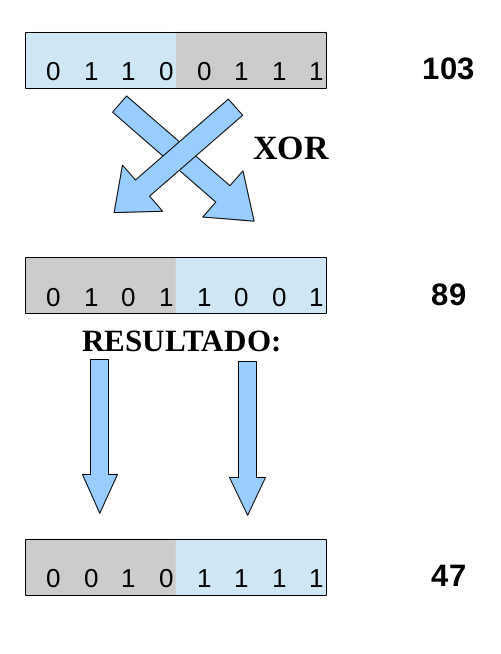
\includegraphics[width=7cm]{es.jpg}
\caption{Esquema de intercambio.}
\label{vovo}
\end{figure}

Un código simplificado (para ocho bits) que hace la operación anterior es el siguiente:
\begin{verbatim}

   char a = 15;
   char temp;
   char temp1;
   char temp2;
   char Xn1;
   char Xn2;
   char Xn3;
   Xn1=103;
   Xn2= 89;
            temp1 = Xn2 & a;
            temp2 = Xn1 >> 4;
            temp = temp1^temp2;
            temp1 = Xn2 >> 4;
            temp2 = Xn1 & a;
            Xn3=(temp1^temp2)<<4;
            Xn3|=temp;
\end{verbatim}


Ahora, para los ejemplos que se muestran aquí se utilizan 32 bits, esto significa que se van a dividir los datos generados por los mapas caóticos en dos partes: cada una de 16 bits. También, en este caso, necesitamos un nuevo valor para a: $(a = 2^{16}-1= 65,535)$


En los casos que se manejan aquí, se ha hecho variar el parámetro $j$  desde 5 hasta 15, recordemos que cuando $i=j$, el mapa es invertible, pero queremos observar cuál es el comportamiento cuando $ i \neq j$.




 
\section{Ejemplos donde varía j.}

\subsection{Procedimiento.}
Se eligieron los siguientes parámetros fijos para el valor de $i$:

\begin{itemize}
\item Mapa 1: $i =  5$.
\item Mapa 2: $i = 14$.
\end{itemize}

También se han elegido los siguientes parámetros fijos para el valor de $q$:

\begin{itemize}
\item Mapa 1: $q = 29.$
\item Mapa 2: $q = 31.$
\end{itemize}


Ahora, es necesario calcular para cada uno de los mapas el valor del parámetro que está dado por la siguiente expresión:
\begin{equation}
\beta = q 2^{n-i}
\end{equation}


Ahora, lo que hacemos es variar la variable $j$,  desde $j=5$ hasta $j=16$, por lo tanto, vamos a tener 12 casos distintos, a continuación, mostramos una tabla de los casos que se han formado.


\begin{table}[H]
\centering
\caption{Casos posibles al variar $j$.}
\begin{tabular}[c]{|c|c|c|c|c|}
\hline

\multicolumn{5}{|c|}{Casos posibles.}\\
\hline
\hline
\multicolumn{5}{|c|}{Caso 1}\\
\hline
Especificación de mapa & Valor de i & Valor de j & Valor de q & Parámetro \\
\hline
Valor mapa 1 &  5  &  5 & 29 & 3892314112\\

\hline
Valor mapa 2 & 14  & 5 & 31 & 8126464\\
\hline
\hline


\multicolumn{5}{|c|}{Caso 2}\\
\hline
Especificación de mapa & Valor de i & Valor de j & Valor de q & Parámetro \\
\hline
Valor mapa 1 &  5  &  6  & 29 & 3892314112\\

\hline
Valor mapa 2 & 14  &  6  & 31 & 8126464\\
\hline
\hline
\multicolumn{5}{|c|}{Caso 3}\\
\hline
Especificación de mapa & Valor de i & Valor de j & Valor de q & Parámetro \\
\hline
Valor mapa 1 &  5  &  7  & 29 & 3892314112\\

\hline
Valor mapa 2 & 14  &  7  & 31 & 8126464\\
\hline
\hline
\multicolumn{5}{|c|}{Caso 4}\\
\hline
Especificación de mapa & Valor de i & Valor de j & Valor de q & Parámetro \\
\hline
Valor mapa 1 &  5  &  8  & 29 & 3892314112\\

\hline
Valor mapa 2 & 14  &  8  & 31 &  8126464 \\
\hline
\hline
\multicolumn{5}{|c|}{Caso 5}\\
\hline
Especificación de mapa & Valor de i & Valor de j & Valor de q & Parámetro \\
\hline
Valor mapa 1 &  5  &  9 & 29 & 3892314112\\

\hline
Valor mapa 2 & 14  & 9 & 31 & 8126464 \\
\hline
\hline
\multicolumn{5}{|c|}{Caso 6}\\
\hline
Especificación de mapa & Valor de i & Valor de j & Valor de q & Parámetro \\
\hline
Valor mapa 1 &  5  &  10  & 29 & 3892314112\\

\hline
Valor mapa 2 & 14  &  10  & 31 & 8126464\\
\hline
\hline
\multicolumn{5}{|c|}{Caso 7}\\
\hline
Especificación de mapa & Valor de i & Valor de j & Valor de q & Parámetro \\
\hline
Valor mapa 1 &  5  &  11 & 29 & 3892314112\\

\hline
Valor mapa 2 & 14  & 11 & 31 & 8126464 \\
\hline
\hline
\multicolumn{5}{|c|}{Caso 8}\\
\hline
Especificación de mapa & Valor de i & Valor de j & Valor de q & Parámetro \\
\hline
Valor mapa 1 &  5  &  12 & 29 & 3892314112\\

\hline
Valor mapa 2 & 14  &  12 & 31 & 8126464\\
\hline
\hline
\multicolumn{5}{|c|}{Caso 9}\\
\hline
Especificación de mapa & Valor de i & Valor de j & Valor de q & Parámetro \\
\hline
Valor mapa 1 &  5  &  13  & 29 & 3892314112\\

\hline
Valor mapa 2 & 14  &  13  & 31 & 8126464\\
\hline
\hline
\multicolumn{5}{|c|}{Caso 10}\\
\hline
Especificación de mapa & Valor de i & Valor de j & Valor de q & Parámetro \\
\hline
Valor mapa 1 &  5  &  14  & 29 & 3892314112\\

\hline
Valor mapa 2 & 14  &  14  & 31 & 8126464\\
\hline
\hline
\multicolumn{5}{|c|}{Caso 11}\\
\hline
Especificación de mapa & Valor de i & Valor de j & Valor de q & Parámetro \\
\hline
Valor mapa 1 &  5  &  15 & 29 & 3892314112\\

\hline
Valor mapa 2 & 14  &  15 & 31 & 8126464\\
\hline
\hline
\multicolumn{5}{|c|}{Caso 12}\\
\hline
Especificación de mapa & Valor de i & Valor de j & Valor de q & Parámetro \\
\hline
Valor mapa 1 &  5  &  16 & 29 & 3892314112\\

\hline
Valor mapa 2 & 14  &  16 & 31 & 8126464\\
\hline
\hline
\end{tabular}
\end{table}



\subsection{Resultados.}

A continuación, se muestran los resultados de las pruebas NIST a cada uno de los ejemplos proepuestos.




\begin{table}[H]
\caption{Resultados de las pruebas de aleatoriedad NIST a los datos caso1.dat .}
\label{caso1}
\begin{center}
\begin{small}
\begin{tabular}{|l|c|r|}
\hline

Prueba Aplicada &  P-Valor & Exito? \\
\hline

Aproximate Entropy    &   0.264344  & $\surd$ \\

Block Frecuency  & 0.0000  &  $X$  \\

Cumulative Sums    &   F:0.369788, R:0.021010  & $\surd$ \\

FFT    &   0.0000 &   $X$      \\

Frecuency     &  0.200106 &  $\surd$   \\

Linear Complexity      & 0.348049 & $\surd$ \\

Longest Run      &   0.287818 &    $\surd$      \\

Non Overlapping Template      & 145 de 148    &     $\surd$          \\

Overlapping Template      &  0.0000  &        $X$       \\

Random Excursions      & 6 de 8  &    $\surd$      \\

Random Excursions Variant & 18 de 18 &     $\surd$    \\

Rank &  0.753924 &      $\surd$      \\

Runs &    0.021936 &     $\surd$        \\

Serial &     2 de 2    &     $\surd$        \\

Universal &      0.235458   &   $\surd$            \\

\hline

\end{tabular}
\end{small}
\end{center}
\end{table}



\begin{table}[H]
\caption{Resultados de las pruebas de aleatoriedad NIST a los datos caso2.dat .}
\label{caso1}
\begin{center}
\begin{small}
\begin{tabular}{|l|c|r|}
\hline

Prueba Aplicada &  P-Valor & Exito? \\
\hline

Aproximate Entropy    &    0.344889 & $\surd$ \\

Block Frecuency  & 0.0000  &  $X$  \\

Cumulative Sums    &   F:0.001261, R:0.021010    & $X$ \\

FFT    &   0.0000 &   $X$      \\

Frecuency     &  0.003571 &  $X$   \\

Linear Complexity      & 0.923814 & $\surd$ \\

Longest Run      &   0.675008 &    $\surd$      \\

Non Overlapping Template      & 146 de 148    &     $\surd$          \\

Overlapping Template      &  0.167187  &       $\surd$        \\

Random Excursions      & 8 de 8  &    $\surd$      \\

Random Excursions Variant & 18 de 18 &     $\surd$    \\

Rank &  0.311869 &      $\surd$      \\

Runs &     0.480999 &     $\surd$        \\

Serial &     2 de 2    &     $\surd$        \\

Universal &      0.234840   &   $\surd$            \\

\hline

\end{tabular}
\end{small}
\end{center}
\end{table}




\begin{table}[H]
\caption{Resultados de las pruebas de aleatoriedad NIST a los datos caso3.dat .}
\label{caso1}
\begin{center}
\begin{small}
\begin{tabular}{|l|c|r|}
\hline

Prueba Aplicada &  P-Valor & Exito? \\
\hline

Aproximate Entropy    &    0.000001 & $X$ \\

Block Frecuency  & 0.0000  &  $X$  \\

Cumulative Sums    &   F:0.0000, R:0.0000    & $X$ \\

FFT    &   0.0000 &   $X$      \\

Frecuency     &  0.000574 &  $X$   \\

Linear Complexity      & 0.060673  & $\surd$ \\

Longest Run      &   0.696738 &    $\surd$      \\

Non Overlapping Template      & 135 de 148    &     $X$          \\

Overlapping Template      &  0.0000 &       $X$        \\

Random Excursions      & 8 de 8  &    $\surd$      \\

Random Excursions Variant & N/A &     $X$    \\

Rank &  0.756964 &      $\surd$      \\

Runs &      0.835550  &     $\surd$        \\

Serial &     2 de 2    &     $\surd$        \\

Universal &       0.061077  &   $\surd$            \\

\hline

\end{tabular}
\end{small}
\end{center}
\end{table}





\begin{table}[H]
\caption{Resultados de las pruebas de aleatoriedad NIST a los datos caso4.dat .}
\label{caso1}
\begin{center}
\begin{small}
\begin{tabular}{|l|c|r|}
\hline

Prueba Aplicada &  P-Valor & Exito? \\
\hline

Aproximate Entropy    &    0.0000 & $X$ \\

Block Frecuency  & 0.0000  &  $X$  \\

Cumulative Sums    &   F:0.000089, R:0.000029   & $X$ \\

FFT    &   0.000000 &   $X$      \\

Frecuency     &  0.000060 &  $X$   \\

Linear Complexity      & 0.418519  & $\surd$ \\

Longest Run      &    0.000000 &    $X$      \\

Non Overlapping Template      & 131 de 148    &     $X$          \\

Overlapping Template      &   0.000000  &       $X$        \\

Random Excursions      & N/A  &    $X$      \\

Random Excursions Variant & N/A &     $X$    \\

Rank &  0.262734 &      $\surd$      \\

Runs &      0.000000  &     $X$        \\

Serial &     0 de 2    &     $X$        \\

Universal &       0.000000 &   $X$            \\

\hline

\end{tabular}
\end{small}
\end{center}
\end{table}



\begin{table}[H]
\caption{Resultados de las pruebas de aleatoriedad NIST a los datos caso5.dat .}
\label{caso1}
\begin{center}
\begin{small}
\begin{tabular}{|l|c|r|}
\hline

Prueba Aplicada &  P-Valor & Exito? \\
\hline

Aproximate Entropy    &    0.0000 & $X$ \\

Block Frecuency  & 0.0000  &  $X$  \\

Cumulative Sums    &   F:0.000089, R:0.000029   & $X$ \\

FFT    &   0.000000 &   $X$      \\

Frecuency     &  0.000060 &  $X$   \\

Linear Complexity      & 0.378629 & $\surd$ \\

Longest Run      &    0.344467 &   $\surd$     \\

Non Overlapping Template      & 136 de 148    &     $X$          \\

Overlapping Template      &   0.000000  &       $X$        \\

Random Excursions      & N/A  &    $X$      \\

Random Excursions Variant & N/A &     $X$    \\

Rank & 0.704232 &      $\surd$      \\

Runs &      0.000000  &     $X$        \\

Serial &     1 de 2    &     $X$        \\

Universal &       0.219296 &   $\surd$            \\

\hline

\end{tabular}
\end{small}
\end{center}
\end{table}





\begin{table}[H]
\caption{Resultados de las pruebas de aleatoriedad NIST a los datos caso6.dat .}
\label{caso1}
\begin{center}
\begin{small}
\begin{tabular}{|l|c|r|}
\hline

Prueba Aplicada &  P-Valor & Exito? \\
\hline

Aproximate Entropy    &    0.0000 & $X$ \\

Block Frecuency  & 0.0000  &  $X$  \\

Cumulative Sums    &   F:0.000077, R:0.000054   & $X$ \\

FFT    &   0.000000 &   $X$      \\

Frecuency     &  0.000125 &  $X$   \\

Linear Complexity      & 0.538981 & $\surd$ \\

Longest Run      &   0.502431 &   $\surd$     \\

Non Overlapping Template      & 145 de 148    &    $\surd$          \\

Overlapping Template      &   0.000001  &       $X$        \\

Random Excursions      & N/A  &    $X$      \\

Random Excursions Variant & N/A &     $X$    \\

Rank &  0.414018  &      $\surd$      \\

Runs &    0.965461 &       $\surd$        \\

Serial &     1 de 2    &     $X$        \\

Universal &        0.602243 &   $\surd$            \\

\hline

\end{tabular}
\end{small}
\end{center}
\end{table}




\begin{table}[H]
\caption{Resultados de las pruebas de aleatoriedad NIST a los datos caso7.dat .}
\label{caso7}
\begin{center}
\begin{small}
\begin{tabular}{|l|c|r|}
\hline

Prueba Aplicada &  P-Valor & Exito? \\
\hline

Aproximate Entropy    &     0.000001 & $X$ \\

Block Frecuency  & 0.000000  &  $X$  \\

Cumulative Sums    &   F:0.000269, R:0.002334   & $X$ \\

FFT    &   0.000000 &   $X$      \\

Frecuency     & 0.001386 &  $X$   \\

Linear Complexity      &  0.855630  & $\surd$ \\

Longest Run      &   0.000000 &   $X$     \\

Non Overlapping Template      & 144 de 148    &    $\surd$          \\

Overlapping Template      &    0.008739   &       $X$        \\

Random Excursions      & N/A  &    $X$      \\

Random Excursions Variant & N/A &     $X$    \\

Rank & 0.083238  &      $\surd$      \\

Runs &     0.765977 &       $\surd$        \\

Serial &     0 de 2    &     $X$        \\

Universal &        0.077582 &   $\surd$            \\

\hline

\end{tabular}
\end{small}
\end{center}
\end{table}



\begin{table}[H]
\caption{Resultados de las pruebas de aleatoriedad NIST a los datos caso8.dat .}
\label{caso8}
\begin{center}
\begin{small}
\begin{tabular}{|l|c|r|}
\hline

Prueba Aplicada &  P-Valor & Exito? \\
\hline

Aproximate Entropy    &     0.000000 & $X$ \\

Block Frecuency  & 0.000000  &  $X$  \\

Cumulative Sums    &   F:0.0000, R:0.0000   & $X$ \\

FFT    &   0.000000 &   $X$      \\

Frecuency     & 0.0000 &  $X$   \\

Linear Complexity      &  0.315138  & $\surd$ \\

Longest Run      &   0.000000 &   $X$     \\

Non Overlapping Template      & 102 de 148    &    $X$          \\

Overlapping Template      &    0.000000   &       $X$        \\

Random Excursions      & N/A  &    $X$      \\

Random Excursions Variant & N/A &     $X$    \\

Rank &  0.481634  &      $\surd$      \\

Runs &     0.0000  &       $X$      \\

Serial &     0 de 2    &     $X$        \\

Universal &        0.000000  &      $X$             \\

\hline

\end{tabular}
\end{small}
\end{center}
\end{table}


\begin{table}[H]
\caption{Resultados de las pruebas de aleatoriedad NIST a los datos caso9.dat .}
\label{caso7}
\begin{center}
\begin{small}
\begin{tabular}{|l|c|r|}
\hline

Prueba Aplicada &  P-Valor & Exito? \\
\hline

Aproximate Entropy    &     0.000000 & $X$ \\

Block Frecuency  & 0.000000  &  $X$  \\

Cumulative Sums    &   F: 0.000014, R:0.000023   & $X$ \\

FFT    &   0.000000 &   $X$      \\

Frecuency     & 0.000019 &  $X$   \\

Linear Complexity      &  0.908233  & $\surd$ \\

Longest Run      &   0.000000 &   $X$     \\

Non Overlapping Template      & 135 de 148    &    $X$          \\

Overlapping Template      &    0.000000   &       $X$        \\

Random Excursions      & N/A  &    $X$      \\

Random Excursions Variant & N/A &     $X$    \\

Rank &  0.906877 &      $\surd$      \\

Runs &     0.0000  &       $X$      \\

Serial &     0 de 2    &     $X$        \\

Universal &        0.038467  &      $\surd$           \\

\hline

\end{tabular}
\end{small}
\end{center}
\end{table}


\begin{table}[H]
\caption{Resultados de las pruebas de aleatoriedad NIST a los datos caso10.dat .}
\label{caso7}
\begin{center}
\begin{small}
\begin{tabular}{|l|c|r|}
\hline

Prueba Aplicada &  P-Valor & Exito? \\
\hline

Aproximate Entropy    &     0.000000 & $X$ \\

Block Frecuency  & 0.000000  &  $X$  \\

Cumulative Sums    &   F: 0.000014, R: 0.000023  & $X$ \\

FFT    &    0.000000   &   $X$      \\

Frecuency     & 0.000019 &  $X$   \\

Linear Complexity      &  0.908233  & $\surd$ \\

Longest Run      &   0.000000 &   $X$     \\

Non Overlapping Template      & 135 de 148    &    $X$          \\

Overlapping Template      &    0.000000   &       $X$        \\

Random Excursions      & N/A  &    $X$      \\

Random Excursions Variant & N/A &     $X$    \\

Rank &  0.906877  &      $\surd$      \\

Runs &     0.0000  &       $X$      \\

Serial &     0 de 2    &     $X$        \\

Universal &        0.038467  &     $\surd$           \\

\hline

\end{tabular}
\end{small}
\end{center}
\end{table}


\begin{table}[H]
\caption{Resultados de las pruebas de aleatoriedad NIST a los datos caso11.dat .}
\label{caso7}
\begin{center}
\begin{small}
\begin{tabular}{|l|c|r|}
\hline

Prueba Aplicada &  P-Valor & Exito? \\
\hline

Aproximate Entropy    &     0.000000 & $X$ \\

Block Frecuency  & 0.000000  &  $X$  \\

Cumulative Sums    &   F:0.0000, R:0.0000   & $X$ \\

FFT    &   0.000000 &   $X$      \\

Frecuency     & 0.0000 &  $X$   \\

Linear Complexity      & 0.234100 & $\surd$ \\

Longest Run      &   0.000000 &   $X$     \\

Non Overlapping Template      & Failure   &    $X$          \\

Overlapping Template      &    0.000000   &       $X$        \\

Random Excursions      & N/A  &    $X$      \\

Random Excursions Variant & N/A &     $X$    \\

Rank &  0.000000  &      $X$     \\

Runs &     0.0000  &       $X$      \\

Serial &     0 de 2    &     $X$        \\

Universal &        0.000000  &      $X$             \\

\hline

\end{tabular}
\end{small}
\end{center}
\end{table}


\begin{table}[H]
\caption{Resultados de las pruebas de aleatoriedad NIST a los datos caso12.dat .}
\label{caso7}
\begin{center}
\begin{small}
\begin{tabular}{|l|c|r|}
\hline

Prueba Aplicada &  P-Valor & Exito? \\
\hline

Aproximate Entropy    &     0.000000 & $X$ \\

Block Frecuency  & 0.000000  &  $X$  \\

Cumulative Sums    &   F:0.0000, R:0.0000   & $X$ \\

FFT    &   0.000000 &   $X$      \\

Frecuency     & 0.0000 &  $X$   \\

Linear Complexity      &  0.00000  & $X$  \\

Longest Run      &   0.000000 &   $X$     \\

Non Overlapping Template      & FAILURE    &    $X$          \\

Overlapping Template      &    0.000000   &       $X$        \\

Random Excursions      & N/A  &    $X$      \\

Random Excursions Variant & N/A &     $X$    \\

Rank &  0.000000  &    $X$       \\

Runs &     0.0000  &       $X$      \\

Serial &     0 de 2    &     $X$        \\

Universal &        0.000000  &      $X$             \\

\hline

\end{tabular}
\end{small}
\end{center}
\end{table}




\section{Conclusiones.}

Los mejores caso fueron del caso 1 al caso 3. A partir de ese momento, no se obtuvieron buenos resultados. De acuerdo a los resultados obtenidos se puede concluir que no es recomendable que los mapas que participan en la operación indicada, tengan el mismo valor para j, como se hizo en estas pruebas.

Conforme el valor de j aumenta, los resultados empeoran, como ocurre con las últimas pruebas mostradas.



\end{document}


